
\section{Files and Functions}
Up to this point everything can be run from the ''Command Window.''
 Now we'll start branching into containing your code in files.
 There are two types of files that matlab considers code, \emph{Scripts} and \emph{Functions}.
 Both have the same .m file extension, but are treated differently by Matlab.
 
Functions and scripts are a great way of ''reusing'' code.
 If you find yourself frequently entering the same code, then perhaps it should be a function or script.
 Scripts can operate on whatever variables you are currently working with, and they leave you with all of the variables they used.
 Functions on the other hand, only know what you send them, and return only what you want.

\subsection{Scripts}
A script is simply a collection of commands in a file.
 When you run a script you can think of it as running within the command window itself.
 
To create a script, simply save a file of commands as a text file with a .m extension.
 All of the examples in the previous chapters have been scripts, and as a reminder you can download them from \href{https://github.com/KEClaytor/QuickDirtyMatlab/tree/master/code}{Github}.

\begin{quote}
\verbatiminput{code/ch03_script.m}
\end{quote}

\pagebreak
\subsection{Cells}
You don't have to run an entire script at once.
 From the editor, you can select a few lines and then use the F9 key to run those.
 You can also split your code into ''cells'' with ''\%\%''.
 Each cell can be run with Ctrl-Enter.
 You can run a cell and move to the next with Shift-Ctrl-Enter.

\begin{quote}
\verbatiminput{code/ch03_cell.m}
\end{quote}

\pagebreak
\subsection{Functions}
A function is set of commands that takes in some variables, and returns another set.
 The only variables the function can see are those that have been sent into it.
 In Matlab parlance, this means the function has it's own ''workspace''.
  
You have already seen functions in the operators such as $\sin()$ and $\cos()$.
 You will call your own functions in the same way (see Subfunctions for an example).
 
It is good practice to name the file the same name as the function that is in it.
 This helps matlab find the appropriate function.
 Consider the ambiguity of two files named differently but with the same content.
 Which should be used?

The defining characteristic of a function is the line;
\begin{verbatim}
 function [out]=function_name(in)
\end{verbatim}

Here's how it looks in context.
\begin{quote}
\verbatiminput{code/ch03_fibfunc.m}
\end{quote}

If there is only one output to your function you can assign it directly;
\begin{verbatim}
 x = multiplybythree(4);
\end{verbatim}

You can use brackets to assign multiple outputs.
\begin{verbatim}
 [x,y] = two_outputs_of_n(n);
\end{verbatim}

You can ignore an output with the $~$ character.
\begin{verbatim}
 [x,~,z] = you_only_want_the_first_and_third(a,b,c)
\end{verbatim}

\pagebreak
\subsection{Subfunctions}
As mentioned above, you can use functions inside of functions.
 If you have a simple function call that does not need to be repeated, you can contain it as a subfunction.
 This is visible only to the functions that also appear in this file.

\begin{quote}
\verbatiminput{code/ch03_fibsubfunc.m}
\end{quote}


\pagebreak
\subsection{The Path}
How does Matlab find your functions?
 They can be in one of two places; the current directory or the path.
 The path stores the list of files Matlab looks through in order to find functions and scripts.
 Here's what it looks like in R2013a:

\begin{figure}[ht!]
\centering
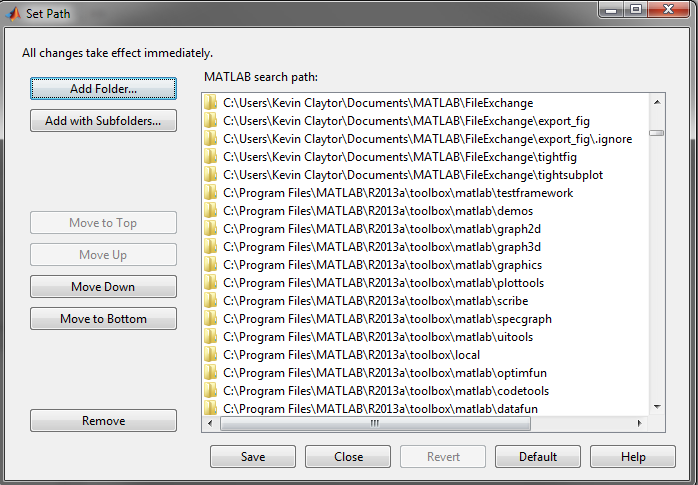
\includegraphics[width=90mm]{img/path.png}
\caption{The Matlab path window.}
\label{overflow}
\end{figure}